%%This is a very basic article template.
%%There is just one section and two subsections.
\documentclass[a4paper,12pt]{article}
\usepackage[english]{babel}
\usepackage{amsmath}
\usepackage{amssymb}
\usepackage{amsthm}

% Graphics
\usepackage{graphicx}
\graphicspath{{img/}}
\DeclareGraphicsExtensions{.eps,.png,.pdf,.jpg}

% Windows-only
\usepackage[utf8]{inputenc}
\usepackage{epstopdf}
%pdf latex -synctex=1 --shell-escape -interaction=nonstopmode --src-specials

\usepackage[ttscale=.875]{libertine}

% Display
\usepackage[font={small,it}]{caption}
%\usepackage{multirow}
%\usepackage{fancyvrb}
%\usepackage{listings}

% Illustrations
%\usepackage{tikz}
%usetikzlibrary{arrows,automata}

% Algorithms
%\usepackage{algorithm}
%\usepackage{algpseudocode}

% For bibliography
\usepackage{url}

% \usepackage{setspace}
\usepackage{geometry}
\geometry{%
	top=25mm, bottom=30mm,
	left=25mm, right=30mm, twoside
}

\setlength{\parskip}{8pt}
\setlength{\parindent}{0cm}

\newlength{\myleftmargin}
\setlength{\myleftmargin}{-6ex}
\newlength{\fixboxwidth}
\setlength{\fixboxwidth}{\marginparwidth}
\addtolength{\fixboxwidth}{\myleftmargin}
\newcommand{\fix}[1]{\marginpar{%
    \fbox{\parbox{\fixboxwidth}{\footnotesize \red{#1}}}}}

%%%%%%%%%%%%%%%%%%%%%%%%%% Text commands
\usepackage{color}
\definecolor{emph}{rgb}{.1,.4,.1}
\definecolor{dark-red}{rgb}{0.4,0.15,0.15}
\definecolor{dark-blue}{rgb}{0.15,0.15,0.4}
\definecolor{medium-blue}{rgb}{0,0,0.5}
\newcommand{\ow}[1]{``\emph{#1}''}%\textcolor{emph}{\emph{#1}}
\newcommand{\e}[1]{\emph{#1}}
%\newcommand{\red}[1]{\textcolor{red}{#1}}
%\newenvironment{redp}{\par\color{red}}{\par}

%%%%%%%%%%%%%%%%%%%% Figure stuff
\newenvironment{myfig}[2]{%
\def\mystupidworkaround{#1}
\def\mystupidworkaroundtwo{#2}
\begin{center}
}{%
	\captionof{figure}{\mystupidworkaroundtwo}
  	\label{\mystupidworkaround}
\end{center}
}
% \usepackage{float}
% \newenvironment{myfig}[2]{%
% \def\mystupidworkaround{#1}
% \def\mystupidworkaroundtwo{#2}
% \begin{figure}[H]
% 	\centering
% }{%
%  	\caption{\mystupidworkaroundtwo}
%  	\label{\mystupidworkaround}
% \end{figure}
% }

% % MathBBM / MathCal symbols
\newcommand{\R}{\mathbb{R}}
\newcommand{\N}{\mathbb{N}}
\newcommand{\D}{\mathcal{D}}
\renewcommand{\P}{\mathcal{P}}
\renewcommand{\L}{\mathcal{L}}
\newcommand{\Udeim}{\mathcal{U}}
\newcommand{\E}{\mathcal{E}}
\newcommand{\V}{\mathcal{V}}
\newcommand{\W}{\mathcal{W}}
\newcommand{\Rp}{\mathbb{R}_+}

%%%%%%%%%%%%%%%%%%%%%%%% Dimensions
% State space: d
\def\dis{l} % input space
\def\dos{k} % output space
\def\dpar{p} % parameter space

%%%%%%%%%%%%%%%%%%%%%%%% Kernel related 
\newcommand{\K}{K}
\renewcommand{\H}{\mathcal{H}}
\newcommand{\Pxdot}{\K(\vx,\cdot)}
\newcommand{\Pydot}{\K(\vy,\cdot)}
\newcommand{\Pxidot}{\K(\vx_i,\cdot)}
\newcommand{\Pxjdot}{\K(\vx_j,\cdot)}
\newcommand{\Pyidot}{\K(\vy_i,\cdot)}
\newcommand{\Kxix}{\K(\vx_i,\vx)}
\newcommand{\spH}[2]{\sp{#1}{#2}_{\H}}
\newcommand{\spHq}[2]{\sp{#1}{#2}_{\H^q}}
\newcommand{\noH}[1]{\norm{#1}{\H}}
\newcommand{\noHq}[1]{\norm{#1}{\H^q}}
\newcommand{\Kh}{\tilde{\K}}
\newcommand{\vci}{\vc_i}

%%%%%%%%%%%%%%%%%%%%%%%% Vectors and Matrices
\newcommand{\mx}[1]{\ensuremath{\left(\begin{matrix}#1\end{matrix}\right)}}
\newcommand{\sm}[1]{\ensuremath{\left(\begin{smallmatrix}#1\end{smallmatrix}\right)}}
\newcommand{\makebf}[1]{\boldsymbol{#1}}
\newcommand{\vnull}{\makebf{0}}
\newcommand{\vone}{\makebf{1}}
\newcommand{\vA}{\makebf{A}}
\newcommand{\vB}{\makebf{B}}
\newcommand{\vC}{\makebf{C}}
\newcommand{\vD}{\makebf{D}}
\newcommand{\vE}{\makebf{E}}
\newcommand{\vF}{\makebf{F}}
\newcommand{\vG}{\makebf{G}}
\newcommand{\vH}{\makebf{H}}
\newcommand{\vI}{\makebf{I}}
\newcommand{\vJ}{\makebf{J}}
\newcommand{\vK}{\makebf{K}}
\newcommand{\vL}{\makebf{L}}
\newcommand{\vM}{\makebf{M}}
\newcommand{\vN}{\makebf{N}}
\newcommand{\vP}{\makebf{P}}
\newcommand{\vQ}{\makebf{Q}}
\newcommand{\vR}{\makebf{R}}
\newcommand{\vS}{\makebf{S}}
\newcommand{\vU}{\makebf{U}}
\newcommand{\vV}{\makebf{V}}
\newcommand{\vW}{\makebf{W}}
\newcommand{\vX}{\makebf{X}}
\newcommand{\vY}{\makebf{Y}}
\newcommand{\va}{\makebf{a}}
\newcommand{\vb}{\makebf{b}}
\newcommand{\vc}{\makebf{c}}
\newcommand{\ve}{\makebf{e}}
\newcommand{\vf}{\makebf{f}}
\newcommand{\vg}{\makebf{g}}
\newcommand{\vj}{\makebf{j}}
\newcommand{\vk}{\makebf{k}}
\newcommand{\vn}{\makebf{n}}
\newcommand{\vp}{\makebf{p}}
\newcommand{\vq}{\makebf{q}}
\newcommand{\vr}{\makebf{r}}
\newcommand{\vu}{\makebf{u}}
\newcommand{\vv}{\makebf{v}}
\newcommand{\vw}{\makebf{w}}
\newcommand{\vx}{\makebf{x}}
\newcommand{\vy}{\makebf{y}}
\newcommand{\vz}{\makebf{z}}
\newcommand{\val}{\makebf{\alpha}}
\newcommand{\vmu}{{\makebf{\mu}}}
\newcommand{\vxi}{\makebf{\xi}}
\newcommand{\veta}{\makebf{\eta}}
\newcommand{\vSig}{\makebf{\Sigma}}
\newcommand{\vLam}{\makebf{\Lambda}}

% Tilde: Projected quantities 
\newcommand{\vtA}{\tilde{\vA}}
\newcommand{\vtB}{\tilde{\vB}}
\newcommand{\vtC}{\tilde{\vC}}
\newcommand{\vtJ}{\tilde{\vJ}}
\newcommand{\vtM}{\tilde{\vM}}
\newcommand{\vtQ}{\tilde{\vQ}}
\newcommand{\vtU}{\tilde{\vU}}
\newcommand{\vtV}{\tilde{\vV}}
\newcommand{\vtc}{\tilde{\vc}}
\newcommand{\vtq}{\tilde{\vq}}
\newcommand{\vtx}{\tilde{\vx}}
\newcommand{\vtv}{\tilde{\vv}}
\newcommand{\vtz}{\tilde{\vz}}
\newcommand{\tf}{\tilde{f}}
\newcommand{\tlambda}{\tilde{\lambda}}

% Hat: Approximated quantities
\newcommand{\hf}{\hat{f}}
\newcommand{\vhf}{{\hat{\vf}}}
\newcommand{\vhV}{{\hat{\vV}}}
\newcommand{\vhW}{{\hat{\vW}}}
\newcommand{\vhP}{\hat{\vP}}
\newcommand{\vhR}{{\hat{\vR}}}
\newcommand{\vhU}{\hat{\vU}}

% Tilde hat: Projected approximated quantities
\newcommand{\vthf}{\tilde{\vhf}}

%%%%%%%%%%%%%%%%%%%%%%%% Misc
\renewcommand{\O}[1]{\ensuremath{\mathcal{O}\left(#1\right)}}
\newcommand{\bs}{\backslash}
\newcommand{\fo}{~\forall~}
\newcommand{\ex}{~\exists~}
\newcommand{\exu}{~\exists!~}
\newcommand{\ep}{\epsilon}
\newcommand{\es}{\emptyset}
\newcommand{\norm}[2]{\left|\left|#1\right|\right|_{#2}}
\newcommand{\no}[1]{\norm{#1}{}}
\newcommand{\noG}[1]{\norm{#1}{G}}
\newcommand{\Mmo}{\mathcal{C}}
\newcommand{\mmo}{\mathcal{D}}
\newcommand{\PM}{\P_{\Mmo}}
\newcommand{\Pm}{\P_{\mmo}}
\newcommand{\flux}{f}%
\newcommand{\sat}{s}%s^{\ep,\tau}
\newcommand{\col}{p{2cm}}

\renewcommand{\sp}[2]{\left\langle #1,#2 \right\rangle}
\newcommand{\spG}[2]{\sp{#1}{#2}_{G}}
% \newcommand{\spHq}[2]{\sp{#1}{#2}_{\H^q}}
\newcommand{\Ball}[2]{B_{#1}\left(#2\right)}

%%%%%%%%%%%%%%%%%%%%%%%%% Sizes
\newcommand{\single}{.8\textwidth} % 1 image in row
\newcommand{\third}{.32\textwidth}
\newcommand{\half}{.49\textwidth}
\newcommand{\quarter}{.24\textwidth}

%%%%%%%%%%%%%%%%%%%%%%%%% Sums, integrals, limits 
\newcommand{\suml}[2]{\sum\limits_{#1}^{#2}}
\newcommand{\sumi}{\suml{i=1}{N}}
\newcommand{\sumim}{\suml{i=1}{m}}
\newcommand{\sumj}{\suml{j=1}{N}}
\newcommand{\sumk}{\suml{k=1}{N}}
\newcommand{\sumjq}{\suml{j=1}{q}}
\newcommand{\sumr}{\suml{i=1}{r}}
\newcommand{\sumjk}{\suml{j=1}{k}}
\newcommand{\sumik}{\suml{j=1}{k}}
\newcommand{\sumkM}{\suml{k=1}{M}}
\newcommand{\intl}[2]{\int\limits_{#1}^{#2}}

%%%%%%%%%%%%%%%%%%%%%%%%%% SVR-Commands
\newcommand{\ap}{\val^+}
\newcommand{\am}{\val^-}
\newcommand{\aip}{\alpha_i^+}
\newcommand{\aim}{\alpha_i^-}
\newcommand{\ajp}{\alpha_j^+}
\newcommand{\ajm}{\alpha_j^-}
\newcommand{\apm}{\ap-\am}
\newcommand{\apmb}{\left(\ap-\am\right)}
\newcommand{\dw}{\nabla W}
\newcommand{\dwp}{\dw^+(\ap,\am)}
\newcommand{\dwpi}{\dw_i^+(\ap,\am)}
\newcommand{\dwpj}{\dw_j^+(\ap,\am)}
\newcommand{\dwm}{\dw^-(\ap,\am)}
\newcommand{\dwmi}{\dw_i^-(\ap,\am)}
\newcommand{\dwmj}{\dw_j^-(\ap,\am)}
\newcommand{\vdw}{\nabla \vW}
\newcommand{\clip}[3]{\left[#1\right]^{#2}_{#3}}
\newcommand{\nonp}[1]{\norm{#1}{\Np}}
\newcommand{\ripp}{r_i^{++}}
\newcommand{\sjpp}{s_j^{++}}
\newcommand{\xip}{\xi_i^+}
\newcommand{\xim}{\xi_i^-}
\newcommand{\noep}[1]{\left|#1\right|_\ep}
\newcommand{\wplus}{\nabla\vw^+} 
\newcommand{\wm}{\nabla\vw^-}

%%%%%%%%%%%%%%%%%%%%%%%%%% VKOGA-Commands
\newcommand{\tp}{\tilde{\phi}}
\newcommand{\sfx}{{s_{f,X}}}
\newcommand{\sfxm}{{s_{f,X_m}}}
\newcommand{\Pq}{\P^q}
\newcommand{\PHX}{\P_{\H^X}}
%\newcommand{\PHXq}{\Pq_{\H^X}}
\newcommand{\Kinj}{(\vK^{-1})_j^T}
\newcommand{\OX}{\Omega_X}
\newcommand{\OXm}{\vx\in\Omega\bs\Omega_{X_{m-1}}}
\newcommand{\nKx}{\nabla\vK(\vx)}
\newcommand{\gxf}{G_{X,\vf}} % vectorial gain function
\newcommand{\px}{\phi_{\vx}}
\newcommand{\pxv}{\px^{\nabla v}}
\newcommand{\tpx}{\tp_{\vx}}
\newcommand{\tpv}{\tp^{\nabla v}}
\newcommand{\vtpx}{\makebf{\tp}_{\vx}}
\newcommand{\tpxv}{\tpx^{\nabla v}}
\newcommand{\tN}{\tilde{N}}
\newcommand{\im}{{i_{max}}}

%%%%%%%%%%%%%%%%%%%%%% DEIM commands
\newcommand{\ei}{{\wp_i}}
\newcommand{\DEI}{\DE_{EI}}
\newcommand{\DEIJ}{\DE}
\newcommand{\Prm}{\Pi_m}
\newcommand{\Pmd}{\Pi_{m'}}
\newcommand{\proj}{\bigl(\vI - \vV\vW^T\bigr)}

%%%%%%%%%%%%%%%%%%%%%% Operators
\DeclareMathOperator{\rangeop}{range}
\DeclareMathOperator{\meanop}{mean}
\DeclareMathOperator{\sgn}{sign}
\DeclareMathOperator{\diagmat}{diag}
\DeclareMathOperator{\divop}{div}
\newcommand{\sign}[1]{\sgn\left(#1\right)}
\newcommand{\range}[1]{\rangeop\left(#1\right)}
\newcommand{\diag}[1]{\diagmat\left(#1\right)}
\renewcommand{\d}[2]{\frac{\partial #1}{\partial #2}}
\newcommand{\dx}{\partial_x}%
\newcommand{\dd}[2]{\frac{\partial^2 #1}{\partial {#2}^2}}

%%%%%%%%%%%%%%%%%%%%%% Error estimation
\newcommand{\intt}{\intl{0}{t}}
\newcommand{\exo}{E_0} % initial error
\newcommand{\exomu}{\exo(\vmu)}
\newcommand{\ea}{E_A} % approximation error
\newcommand{\eproj}{\left(\vI-\vV\vW^T\right)} %projection error
\newcommand{\fd}{{h_{X,\Omega}}} % fill distance
\renewcommand{\Ball}[2]{\overline{B_{#1}\left(#2\right)}}
\newcommand{\Bts}{\Ball{\Theta}{s}}
\newcommand{\Bty}{\Ball{\Theta}{y}}
\newcommand{\Bf}{\mathcal{B}} % bell functions
\newcommand{\DE}{\Delta}
\newcommand{\DGLE}{\DE_{GLE}}
\newcommand{\DLSLE}{\DE_{LSLE}} 
\newcommand{\Gno}{\Gamma_1^c}

%%%%%%%%%%%%%%%%%%%% Code
\newcommand{\ML}{\textsc{MatLab}}%{\tiny\texttrademark~}
\newcommand{\KM}{\textit{KerMor}}
\newcommand{\code}[1]{\lstinline$#1$}
\definecolor{c-keywords}{rgb}{.1,.1,.5}
\definecolor{c-identifier}{rgb}{0.3,0.3,0.3}

% \usepackage{verbatim}
% \lstset{language=Matlab,
% 	basicstyle=\normalsize\ttfamily,
% 	keywordstyle=\bfseries\ttfamily\color{c-keywords},
% 	identifierstyle=\color{c-identifier},
% 	commentstyle=\color{green},
% 	stringstyle=\ttfamily,
% 	showstringspaces=false,
% 	fancyvrb=true,
% 	xleftmargin=5pt,
% 	morekeywords={doc,help,methods,events,properties,abstract,
%                       classdef,double,true,false,this,access,setaccess,getaccess,
% 		      varargin, varargout}
% }
 
% %%%%%%%%%%%%%%%%%%%%%%%%%%%%%%%%%%%%%%%%%%%%%%%%%%%%%%%%%%%%%%%%%%%%%
% %% THEOREM & LEMMA COMMANDS
% %%%%%%%%%%%%%%%%%%%%%%%%%%%%%%%%%%%%%%%%%%%%%%%%%%%%%%%%%%%%%%%%%%%%%
\newtheorem{theorem}{Theorem}[section]
\newtheorem{lemma}[theorem]{Lemma}
\newtheorem{corollary}[theorem]{Corollary}
\newtheorem{proposition}[theorem]{Proposition}
 	
% Option 1: Continuous numbering also for defs & remarks
\theoremstyle{definition}
\newtheorem{definition}[theorem]{Definition}
\theoremstyle{remark}
\newtheorem{remark}[theorem]{Remark}
% 	% Option 2: Own counters for defs & remarks
% 	\theoremstyle{definition}
% 	\newtheorem{definition}{Definition}[section]
% 	\theoremstyle{remark}
% 	\newtheorem{remark}{Remark}[section]
% 	
% 	%\newtheorem{example}[theorem]{Example}
% 	%\newtheorem{xca}[theorem]{Exercise}

\newcommand{\Nk}{\mathcal{N}_k}
\newcommand{\Or}{\Omega_0}
\newcommand{\Om}{\Omega_R}
\newcommand{\intor}{\intl{\Or}{}}
\newcommand{\intom}{\intl{\Om}{}}
\newcommand{\intorb}{\intl{\partial\Or}{}}
\newcommand{\vT}{\makebf{T}}
\newcommand{\vt}{\makebf{t}}
\newcommand{\vsig}{\makebf{\sigma}}
\newcommand{\vSi}{\vS^{iso}}
\newcommand{\vSa}{\vS^{aniso}}
\newcommand{\vSf}{\vS^{act}}
\newcommand{\vPi}{\vP^{iso}}
\newcommand{\vPa}{\vP^{aniso}}
\newcommand{\vPf}{\vP^{act}}
\newcommand{\Sfun}{\makebf{\Upsilon}}
\newcommand{\force}{\vG}
\DeclareMathOperator{\divergence}{\nabla}
\DeclareMathOperator{\tr}{tr}
\DeclareMathOperator{\supp}{supp}
\DeclareMathOperator{\grad}{grad}
\renewcommand{\div}[1]{\divergence\cdot\left(#1\right)}
\newcommand{\m}[1]{\ensuremath{\left(\begin{matrix}#1\end{matrix}\right)}}
\newcommand{\sumnk}{\suml{i\in{\Nk}}{}}
\newcommand{\sumgp}{\suml{p=1}{G}}
\newcommand{\jmp}{J^m_p}
\newcommand{\re}[1]{\stackrel{\eqref{#1}}{=}}
\newcommand{\sumvk}{\suml{m\in V_k}{}}
\newcommand{\pmp}{X^m_p}%\Phi_m(X_p)
\usepackage{mathtools}
\DeclarePairedDelimiter{\ceil}{\lceil}{\rceil}
%\newcommand{\sm}[1]{\ensuremath{\left(\begin{smallmatrix}#1\end{smallmatrix}\right)}}

\allowdisplaybreaks
\begin{document}

As perspective, we will work on the \e{reference configuration} regarding all quantities and relate to the \e{current configuration} only where necessary.
The quantities referred to in the reference configuration are upper-case letters and we denote quantities in the reference configuration by lower-case letters.
Bold face is used to indicate vectorial quantities.

We model the movement/deformation of a continuous muscle over time, whose shape corresponds to the reference domain $\Or\subset\R^3$.
The movement of each particle $X\in\R^3$ in the body is described by a \e{motion} $\chi(X,t)\in\R^3$, which gives the position of each $X\in\R^3$ at time
$t\in[0,T]$ with $\Or = \chi(\Or,0)$.

We define the quantities
\begin{align}
	\text{velocity field} && \vV(X,t) &:= \d{\chi}{t}(X,T),\\
	\text{acceleration field} && \vA(X,t) &:= \d{\vV}{t}(X,t) = \dd{\chi}{t}(X,t),\\
	\text{deformation gradient} && \vF(X,t) &:= \d{\chi}{X}(X,t) = \m{\nabla \chi_1 & \nabla \chi_2 & \nabla \chi_3}^T \in \R^{3\times 3},\\
	\text{right cauchy strain tensor} && \vC(X,t) &:= \vF(X,t)^T\vF(X,t)\\
	\text{volume ratio} && J(X,t) &:= \det(\vF(X,t)).
\end{align}

\section{Derivation of governing equations}
Assuming a density $\rho_0(X), \left[\rho_0(X)\right] = \frac{kg}{mm^3}$ at each point we define the total momentum
\begin{align*}
 	\vL(t) &:= \intor \rho_0(X)\vV(X,t) dX, & [\vL(t)] &= [\rho_0\vV]mm^3 = \frac{kg}{mm^3}\frac{m}{s}mm^3 = 10^{-3}Nms
\end{align*} 
for which we postulate the balance equation
\begin{align}
	\force(t) \stackrel{!}{=} \d{\vL}{t}(t) = \vL'(t) = \intor \rho_0(X)\d{\vV}{t}(X,t) dX = \intor \rho_0(X)\vA(X,t) dX,\label{def:bal_eq}
\end{align}
given \e{resultant forces} $\force(t)$.

\subsection{Structure of force}
We assume the forces $\force(t)$ to be composed of two different sources: Forces on the boundary and body forces.
The body forces $\vB(X,t)$ measures the force per unit reference volume ($\left[\vB(X,t)\right] = 10^{-3}\frac{N}{mm^3}$) on $X$ at time $t$.
These forces are self-weight or gravity, for example.
Further, we assume to have \e{traction vectors} $\vT(X,t,N)$ (first Piola-Kirchhoff traction vector) that indicates the force working per unit
surface area ($[\vT(X,t,N)] = 10^{-3}\frac{N}{mm^2} = 10^{-3}MPa = kPa$) with normal $N$ at the point $X\in\partial\Or$ at time $t$.
Then the resultant forces are given as
\begin{align}
	\force(t) &:= \intorb \vT(X,t,N)dN + \intor \vB(X,t)dX, & \left[\force(t)\right] = \left[\vL'(t)\right] &= 10^{-3}N = mN. \label{def:force}
\end{align}

According to \e{Cauchy's stress theorem}, we can express tractions as tensor product
\begin{align}
	\vT(X,t,N) &= \vP(X,t)N,\label{def:T}
\end{align}
where $\vP$ denotes the \e{first Piola-Kirchhoff stress tensor}, which is measured in kiloPascal, i.e. $[\vP] = kPa$.
With this we have, following Gauss integral theorem,
\begin{align}
	\intorb \vT(X,t,N)dN &= \intorb \vP(X,t)NdN = \intor \divergence\vP(X,t)dX.\label{eq:div_form_traction}
\end{align}
Using representation \eqref{eq:div_form_traction} in the force composition 
\eqref{def:force} yields the following form of the balance equation \eqref{def:bal_eq}:
\begin{align}
	\intor \rho_0(X)\d{\vV}{t}(X,t) dX &= \intor \divergence\vP(X,t) + \vB(X,t) dX
\end{align}
As this balance must also be satisfied for each subvolume $\Omega_t\subset\Or$, we actually obtain a pointwise or local form as
\begin{align}
	\rho_0(X)\d{\vV}{t}(X,t) &= \divergence\vP(X,t) + \vB(X,t) \qquad \fo X\in\Or\label{def:maineq}
\end{align}

\subsection{Stress tensor definition}
%Most generally, we consider a \e{traction} force $\vt(\vx,\vn)$ at a current point $\vx\in\Omega$ in normal direction $\vn$. 
Generally, one can deal with stress tensors expressed purely on current or reference configuration and hybrids, i.e. two-point versions.
The physically directly interpretable stress tensor is the \e{cauchy stress tensor} $\vsig(\vx,t)$ defined on the current configuration,
denoting the current stress at $\vx$ on the current unit surface orthogonal to $\vn$ at time $t$.
For solids, a description of the stresses w.r.t. the reference configuration is more practical, which is why one defines
\begin{align}
	\vP(X,t) &:= J\vsig\vF^{-T} &&\text{first Piola-Kirchhoff (stress) tensor}\\
	\vS(X,t) &:= \vF(X,t)^{-1}\vP(X,t) = J\vF^{-1}\vsig\vF^{-T} && \text{second Piola-Kirchhoff tensor} \label{def:secondpiola}
\end{align}
Loosely, $\vP(X,t)$ (as a two-point tensor) describes the stresses in the current configuration per unit (undeformed) reference area at a reference point $X$.
The second Piola-Kirchhoff tensor is purely reference-based and describes the stresses in the reference configuration
per unit (undeformed) reference area at a reference point $X$, see \cite[p. 145ff]{Bonet2008}.

Generally, prescribing the stress tensors (in one form or another) will result in different material behaviour.
Usually, this stress somehow depends on the deformation $\vF(X,t)$ and $X$ (in case of inhomogeneous material).

\subsubsection{Hyperelasticity}
In our setting we deal with \e{hyperelastic materials}, which are characterized by the fact that the current stress is only dependent on the
current configuration/deformation at times $0$ and $t$.
By the variational approach, we see that the internal virtual work conjugate of $\vP$ is $\dot{\vF}$,
which allows us to define a \e{elastic potential} or \e{stored strain energy function} as
\begin{align*}
	\Psi_F(\vF(X,t),X) &:= \intl{0}{t}\vP(X,s):\dot{\vF}(X,s)ds,\\
	[\Psi_F] &= kPa = 10^{-3}\frac{N}{mm^2} = 10^{-3}\frac{J}{mm^2 m} = 10^{-6}\frac{J}{mm^3}.
\end{align*}
which denotes the work done by the stresses per unit undeformed volume from initial to current configuration at $t$,
see \cite[p.156]{Bonet2008} or \cite[p.207]{Holzapfel2000}.
Now, by definition, we have
\begin{align}
	\dot{\Psi}_F(\vF(X,t),X) = \vP(X,t):\dot{\vF}(X,t)\label{eq:psif_dt1}
\end{align}
But considering the analytical time derivative of $\Psi_F$ also gives 
\begin{align}
	\d{\Psi_F}{t}(\vF(X,t),X) = \d{\Psi_F}{\vF}(\vF(X,t),X):\d{\vF}{t}(X,t),\label{eq:psif_dt2} 
\end{align}
leads to
\begin{align*}
	0 &= \dot{\Psi}_F(\vF(X,t),X) - \dot{\Psi}_F(\vF(X,t),X)\\
	 &= \vP(X,t):\dot{\vF}(X,t) - \d{\Psi_F}{\vF}(\vF(X,t),X):\dot{\vF}(X,t)\\
	 &= \left(\vP(X,t) - \d{\Psi_F}{\vF}(\vF(X,t),X)\right):\dot{\vF}(X,t)
\end{align*}
As this must hold for any $\vF$ (and hence $\dot{\vF}$) we obtain the relation
\begin{align}
	\vP(X,t) &= \d{\Psi_F}{\vF}(\vF(X,t),X).
\end{align}
This yields a convenient way of specifying a material stress tensor by providing a suitable $\Psi_F$.
As we will consider \e{homogeneous} material, we will omit the direct spatial dependency of $\Psi_F$ on $X$ in the following.

Further, due to the principle of material frame-indifference \cite[p.198]{Holzapfel2000}, any tensor (e.g. $\vP$)
may actually only depend on the rotation-invariant part of $\vF$, i.e. $\Psi_F$ must also be invariant under rigid body rotations.
For any fixed $X,t$ we can decompose $\vF = \vR\vU$ (\cite[p.85]{Holzapfel2000}) with a
\e{rotation} part $\vR$ with $\vR^T\vR = \vI$ and \e{stretch} part $\vU = \vU^T$.
As
\[
	\vC = \vF^T\vF = (\vR\vU)^T\vR\vU = \vU^T\vR^T\vR\vU = \vU\vU = \vU^2, 
\]
one usually defines a $\Psi_C$ depending on $\vC$ instead of $\vF$.

Omitting the $(X,t)$-arguments, consider
\begin{align}
	\vP:\dot{\vF} &= \vF\vS : \dot{\vF} = \tr((\vF\vS)^T\dot{\vF}) = \tr(\vS^T\vF^T\dot{\vF})\\
	&= \vS : (\vF^T\dot{\vF}) = \vS : \frac{1}{2}(\vF^T\dot{\vF} + \vF^T\dot{\vF})  = \vS : \frac{1}{2}(\dot{\vF}^T\vF + \vF^T\dot{\vF})\\
	&= \vS : \frac{1}{2}\dot{\vC} = \frac{1}{2}\vS : \dot{\vC}
\end{align}
We hence can define
\begin{align}
	\Psi_C(\vC(X,t)) &:= \frac{1}{2}\intl{0}{t}\vS(X,s):\dot{\vC}(X,s)ds\\
		& = \intl{0}{t}\vP(X,s):\dot{\vF}(X,s)ds = \Psi_F(\vF(X,t)),
\end{align}
which gives the same strain energy function, albeit defined using $\vC$ instead of $\vF$.
The same argument as with \eqref{eq:psif_dt1}, \eqref{eq:psif_dt2} yields
\begin{align}
	0 &= \left(\frac{1}{2}\vS(X,t) - \d{\Psi_C}{\vC}(\vC(X,t))\right):\dot{\vC}(X,t).\label{eq:secondpiolahyper}
\end{align}
As again $\vC,\dot{\vC}$ is assumed arbitrary we obtain a way to specify $\vS$ via $\Psi_C$ as
\begin{align}
	\vS(X,t) & := 2\d{\Psi_C}{\vC}(\vC(X,t)).
\end{align}
As we will stick with this perspective, we will simply use $\Psi := \Psi_C$ from now on.

\subsubsection{Incompressibility}
Further, we consider \e{incompressible} material, which is expressed by the condition 
\[
	1 = J(X,t) = \det\vF(X,t) = \sqrt{\det\vC(X,t)}\quad\fo X,t.
\]
This especially means
\begin{align}
	0 &= \d{J}{t}(X,t) = \d{}{t}\sqrt{\det\vC(X,t)}\nonumber\\
	&= \d{\sqrt{\det\vC(X,t)}}{\det\vC(X,t)}\d{\det\vC(X,t)}{\vC(X,t)}:\d{\vC}{t}(X,t)\nonumber\\
	&=\frac{1}{2}\frac{1}{\sqrt{\det\vC(X,t)}} \det(\vC(X,t))\vC(X,t)^{-1}:\dot{\vC}(X,t)\nonumber\\
	&=\frac{1}{2}\sqrt{\det\vC(X,t)}\vC(X,t)^{-1}:\dot{\vC}(X,t)\nonumber\\
	&=\frac{1}{2}J(X,t)\vC(X,t)^{-1}:\dot{\vC}(X,t).\label{def:cincompconstr}
\end{align}
Now, comparing equations \eqref{eq:secondpiolahyper} and \eqref{def:cincompconstr} we obtain
\begin{align}
	0 &= \left(\frac{1}{2}\vS(X,t) - \d{\Psi}{\vC}(\vC(X,t)) + \gamma\frac{1}{2}J(X,t)\vC(X,t)^{-1}\right):\dot{\vC}(X,t),\\
	\vS(X,t) &= 2\d{\Psi}{\vC}(\vC(X,t)) + \gamma J(X,t)\vC(X,t)^{-1},\label{def:incompressible_secondpiola}
\end{align}
where $\gamma$ is an arbitrary scalar.
In order to relate this quantity to a physical quantity, we consider the concept of hydrostatic pressure in a small detour.

\paragraph{Relation to hydrostatic pressure}
In the following we omit the $(X,t)$ (or $(x,t)$) arguments for improved readability.
The Cauchy stress tensor $\vsig$ can be split into a \e{volumetric} and \e{deviatoric} part via
\begin{align}
	\vsig &= \underbrace{\vsig - p\vI}_{=:\vsig'} + p\vI, & p &:= \frac{1}{3}\tr\vsig.
\end{align}
The resulting deviatoric part is trace-free, e.g.
\begin{align}
	\tr{\vsig'} &= \tr\left(\vsig - \frac{1}{3}(\tr\vsig)\vI\right) = \suml{i=1}{3}(\vsig_{ii} - \frac{1}{3}\tr\vsig) = \tr\vsig - \tr\vsig = 0.
\end{align}
Here, the scalar $p$ is called the \e{hydrostatic pressure}, $[p] = kPa$.
From the definition \eqref{def:secondpiola} of the second Piola-Kirchhoff stress tensor we obtain the same split for $\vS$
(omitting $X,t$ arguments for readability) via
\begin{align}
	\vS &= J\vF^{-1}\vsig\vF^{-T} = J\vF^{-1}(\vsig' + p\vI)\vF^{-T}\\
		&= J\vF^{-1}\vsig'\vF^{-T} + pJ\vF^{-1}\vF^{-T}\\
		&=: \vS' + pJ\vC^{-1}.
\end{align}
Now, $\vS$ is not necessarily trace-free anymore, but we identify the property
\begin{align}
	\vS' : \vC &= J\vF^{-1}\vsig'\vF^{-T} : \vC = J\tr\bigl(\vF^{-1}\vsig'\vF^{-T}\vC\bigr)\\
		&= J\tr\bigl(\vF^{-1}\vsig'\vF^{-T}\vF^T\vF\bigr) = J\tr\bigl(\vsig'\vF^{-T}\vF^T\vF\vF^{-1}\bigr)\\
		&= \tr\vsig' = 0.
\end{align}
With this an explicit expression for the hydrostatic pressure can be given as
\begin{align}
	\vS : \vC &= (\vS' + pJ\vC^{-1}) : \vC = \vS': \vC + pJ\vC^{-1} : \vC\\
	&= pJ\tr(\vC^{-1}\vC) = pJ\tr(\vI) = 3pJ,\label{def:hydrostaticpressure}
\end{align}
Now using \eqref{def:incompressible_secondpiola} in \eqref{def:hydrostaticpressure} gives
\begin{align}
	p &= \frac{1}{3}J^{-1}\vS : \vC\\
	  &= \frac{1}{3}J^{-1}\left[2\d{\Psi}{\vC}(\vC) + \gamma J\vC^{-1}\right] : \vC\\
	  &= \gamma + \frac{2}{3}J^{-1}\d{\Psi}{\vC}(\vC):\vC,
\end{align}
so $p$ and $\gamma$ coincide if $\d{\Psi}{\vC}(\vC):\vC = 0$.
According to \cite[p. 168]{Bonet2008}, this holds true for a modified $\Psi$ given by
\begin{align}
	\hat{\Psi}(\vC) &:= \Psi(\det(\vC)^{-\frac{1}{3}}\vC)
\end{align}
Now, we can finally write
\begin{align}
	\vS(X,t) = 2\d{\hat\Psi}{\vC}(\vC(X,t)) + p(X,t)J(X,t)\vC^{-1}(X,t).\label{def:secondpiola_pressure}
\end{align}
Note that in general
\begin{align*}
	\d{}{\vC}\det(\vC)^{-\frac{1}{3}}\vC &= -\frac{1}{3}\det(\vC)^{-\frac{4}{3}}\det\vC \vC^{-1} \vC + \det(\vC)^{-\frac{1}{3}}\\
		&=-\frac{1}{3}\det(\vC)^{-\frac{1}{3}} + \det(\vC)^{-\frac{1}{3}}\\
		&=\frac{2}{3}\det(\vC)^{-\frac{1}{3}},
\end{align*}
and hence
\begin{align}
	\d{\hat\Psi}{\vC}(\vC) = \d{\Psi}{\vC}(\det(\vC)^{-\frac{1}{3}}\vC)
	= \frac{2}{3}\det(\vC)^{-\frac{1}{3}}\d{\Psi}{\vC}(\det(\vC)^{-\frac{1}{3}}\vC) \neq \d{\Psi}{\vC}(\vC).  
\end{align}
For the case of incompressible material we have $\det\vC = 1$.
Hence $\hat{\Psi} = \Psi$ and we have the final form of $\vS$ for incompressible hyperelastic material:
\begin{align}
	\vS(X,t) = 2\d{\Psi}{\vC}(\vC(X,t)) + p(X,t)\vC^{-1}(X,t).\label{def:incompressible_secondpiola_pressure}
\end{align}

\subsubsection{(Transversely) isotropic material}
We will also consider \e{isotropic} material, which means the material response is the same, independent from any rotation or translation of
the reference domain.
In other words, the strain energy function $\Psi$ is rotation-invariant, as the definition of stress tensors via derivatives already ensures translation invariance. 
The introduction of \e{fibres} via a fibre direction $\va_0(X)\in\R^3$
in the described material leads to the extended notion of \e{transversely isotropic} material, where
the strain energy function is given as
\[
	\Psi(\vC,\va_0\otimes \va_0),
\]
where the rotation-invariance holds for both arguments.

For any tensor $\vA$ with eigenvalues $\lambda_1,\lambda_2,\lambda_3$ we have the quantities
\begin{align}
	I_1(\vA) &:= \tr\vA = \lambda_1 + \lambda_2 + \lambda_3,\label{def:I1}\\
	I_2(\vA) &:= \frac{1}{2}\left((\tr \vA)^2 - \tr\vA^2\right) = \lambda_1\lambda_2 + \lambda_1\lambda_3 + \lambda_2\lambda_3,\\
	I_3(\vA) &:= \det\vA = \lambda_1\lambda_2\lambda_3,\label{def:I3}\\
	I_4(\vA,\vv) &:= \vv\cdot\vA\vv = \vA : (\vv \otimes \vv)\label{def:I4} =: \lambda^2_{\vv},\\
	I_5(\vA,\vv) &:= \vv\cdot\vA^2\vv,\label{def:I5}
\end{align}
called \e{invariants}, as they are not changing if $\vA$ is rotated by any proper orthogonal matrix.
For \e{symmetric} $\vA$ we have the derivatives of the invariants given as
\begin{align}
	\d{I_1}{\vA}(\vA) &:= \d{\tr\vA}{\vA}(\vA) = \d{\vI:\vA}{\vA}(\vA) = \vI\\
	\d{I_2}{\vA}(\vA) &:= I_1(\vA)\vI - \vA\\
	\d{I_3}{\vA}(\vA) &:= I_3\vA^{-1}\\
	\d{I_4}{\vA}(\vA,\vv) &:= \vv \otimes \vv\label{def:dI4}\\
	\d{I_5}{\vA}(\vA,\vv) &:= \vv \otimes \vA\vv + \vv\vA \otimes \vv,
\end{align}
see e.g. \cite[p.216/p.268]{Holzapfel2000}.

Now, $\Psi$ can actually be formulated using the invariants \eqref{def:I1}-\eqref{def:I5} as
\[
	\Psi(\vC,\va_0) = \Psi(I_1(\vC),I_2(\vC),I_3(\vC),I_4(\vC,\va_0),I_5(\vC,\va_0)).
\]
for which we have
\begin{align}
	\d{\Psi}{\vC}(I_1,I_2,I_3,I_4,I_5) &=
		\d{\Psi}{I_1}\d{I_1}{\vC} + \d{\Psi}{I_2}\d{I_2}{\vC} + \d{\Psi}{I_3}\d{I_3}{\vC} + \d{\Psi}{I_4}\d{I_4}{\vC} + \d{\Psi}{I_5}\d{I_5}{\vC}\\
		&= \left(\d{\Psi}{I_1} + I_1\d{\Psi}{I_2}\right)\vI - \d{\Psi}{I_2}\vC + I_3\d{\Psi}{I_3}\vC^{-1}\\
		&\quad+ \d{\Psi}{I_4}\va_0\otimes\va_0 + \d{\Psi}{I_5}(\va_0\otimes\vA\va_0 + \va_0\vA\otimes\va_0).
\end{align}

Since we consider incompressible material, $\Psi$ will not depend on the third invariant $I_3 = \det\vC = 1$ as this is already captured in the hydrostatic pressure. 
In the following, we will specify different $\Psi(I_1,I_2,I_4,I_5)$ depending on different invariants to create an additive split as 
\begin{align}
	\vS(X,t) = p(X,t)\vC^{-1}(X,t) + \vSi(X,t) + \vSa(X,t) + \vSf(X,t) +\vSv(X,t) \label{def:S_split}
\end{align}

\subsubsection{Isotropic stress tensor $\vSi$}
Now, for the isotropic part we use (for constants see \cite{Zheng1999})
\begin{align*}
	\Psi(I_1,I_2,I_3) &= c_{10}(I_1-3) + c_{01}(I_2-3), & c_{10} &= 6.352e^{-10}kPa, & c_{01} &= 3.627kPa, 
\end{align*}
which gives
\begin{align}
	\vSi(X,t) &= 2(c_{10} + I_1c_{01})\vI - 2c_{01}\vC(X,t)\\
	\vPi(X,t) &= 2(c_{10} + I_1c_{01})\vF(X,t) - 2c_{01}\vF(X,t)\vC(X,t)
\end{align}

\subsubsection{Anisotropic stress tensor $\vSa$}
Further, we introduce the stretch $\la > 0$ in fibre direction $\va_0(X), \no{\va_0(X)} \equiv 1$, as
\begin{align}
	\la(X,t) &:= \sqrt{I_4(\vC(X,t),\va_0(X))} = \sqrt{\va_0(X)^T\vC(X,t)\va_0(X))}\\
	&= \sqrt{\va_0(X)^T\vF(X,t)^T\vF(X,t)\va_0(X))} = \no{\vF(X,t)\va_0(X)}\label{def:fibrestretch}
\end{align}
Now, according to \cite{Markert2005}, we employ
\begin{align}
	\Psi(\la) := \sumi \frac{b_i}{d_i}(\la^{d_i} - 1) - b_i\ln\la\label{def:markertlaw}
\end{align}
with $n=1$ summands 
\begin{align*}
	b_1 &= 2.756e^{-5}kPa, & d_1 &= 43.373 [-].
\end{align*}
We thus have
\begin{align}
	\d{\Psi}{\vC}(\la) &= \d{\Psi}{\la}(\la)\d{\la}{I_4}(I_4)\d{I_4}{\vC}(\vC,\va_0),\label{eq:dpsidC}
\end{align}
with
\begin{align*}
		 \d{\Psi}{\la}(\la) &= b_1\la^{d_1-1} - b_1\la^{-1} = b_1\la^{-1}(\la^{d_1} - 1),\\
		 \d{\la}{I_4}(I_4) &= \frac{1}{2\sqrt{I_4}} = \frac{1}{2\la}.
\end{align*}
With \eqref{def:dI4} and the above we get
\begin{align*}
	2\d{\Psi}{\vC}(\la) &= 2\left(b_1\la^{-1}(\la^{d_1} - 1)\right) \frac{1}{2\la}\va_0\otimes\va_0
	= \frac{b_1}{\la^2}\left(\la^{d_1} - 1\right) \va_0\otimes\va_0,
\end{align*}
leading to
\begin{align}
	\vSa(X,t) &= \frac{b_1}{\la^2(X,t)}\left(\la^{d_1}(X,t) - 1\right) \va_0(X)\otimes\va_0(X)\\
	\vPa(X,t) &= \frac{b_1}{\la^2(X,t)}\left(\la^{d_1}(X,t) - 1\right) \vF(X,t)\va_0(X)\otimes\va_0(X)
\end{align}

\paragraph{``Numerically improved'' markert law}
The energy density function \eqref{def:markertlaw} has the slight disadvantage
of leading to nonzero derivatives of the effectively applied function $\frac{b_1}{\la^2}\left(\la^{d_1} - 1\right)$ near $\lambda=1$.
As the Markert law is only applicable for $\lambda>1$, quickly increasing parameterizations (e.g. for large $b_1$ and moderate $d_1$, see Figure \ref{fig:steepmarkert})
develop discontinuous derivatives at $\lambda=1$. This is numerically problematic the stiffer the material modeled is.
\begin{figure}[!ht]
	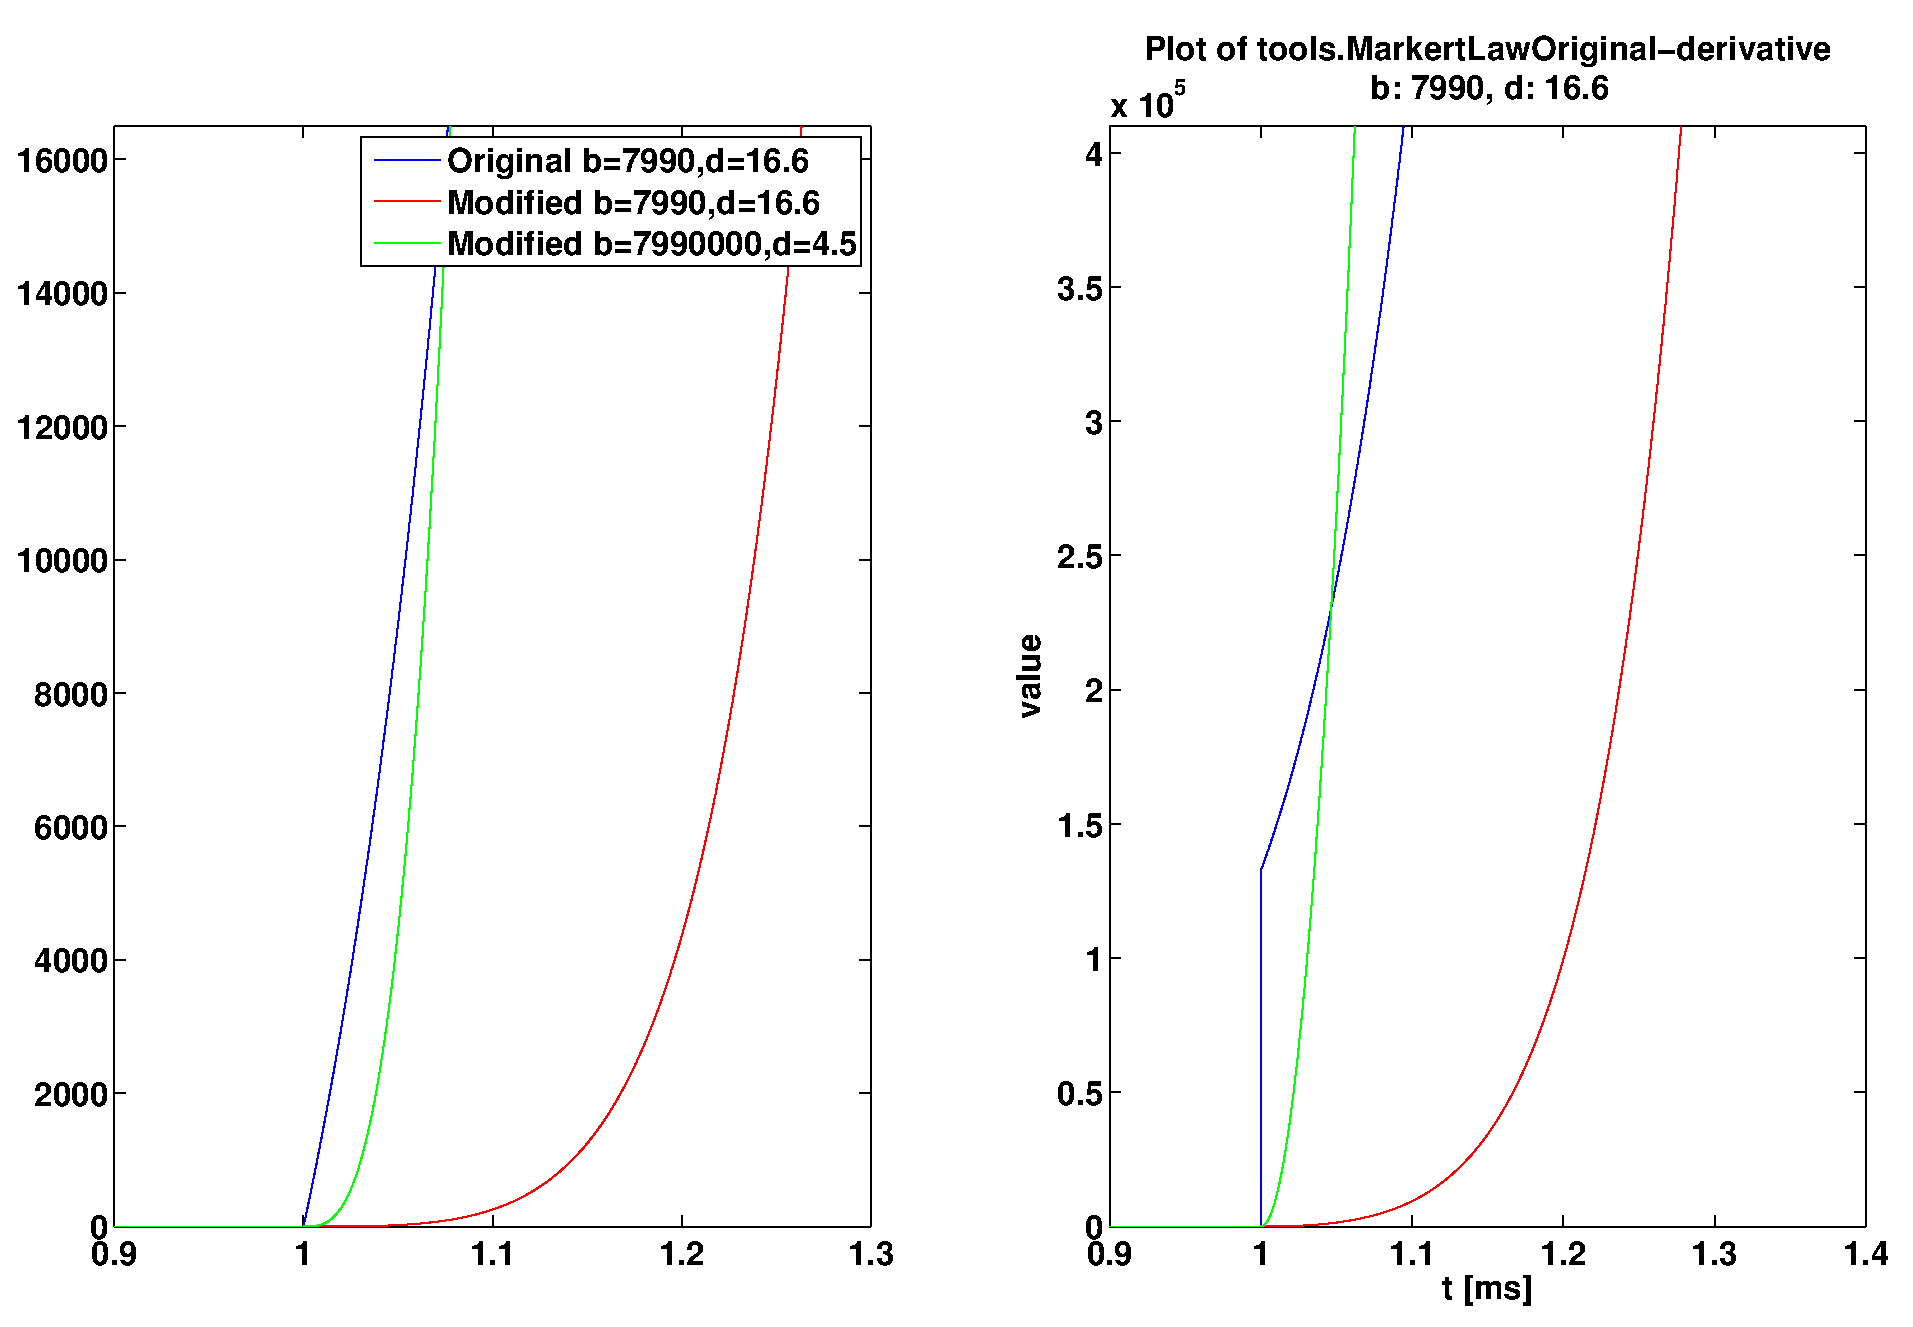
\includegraphics[width=\textwidth]{MarkertLawOriginal}
	\caption{Markert law for $b_1=7990 [kPa]$ and $d_1=16.6 [-]$. Discontinuous derivative at $\lambda=1$ with gap size $b_1d_1=132634 [kPa]$}
	\label{fig:steepmarkert}
\end{figure}

\subsubsection{Active force tensor $\vSf$}\label{sec:active_force}
We further assume to have a muscle activation $\alpha(X,t) \in [0,1]$, which is given by manual settings or motorunit models.
We then define
\begin{align}
	\Psi(\la) &:= \intl{0}{\la} p^{act}(s)ds,\nonumber\\
	p^{act}(\la) &:= p^{max}f_l(\la)f_v(\dla)\alpha(X,t),\nonumber\\
	f_l(\la) &:= \begin{cases}
		-\frac{25}{4}\left(\frac{\la}{\lfo}\right)^2 + \frac{25}{2}\frac{\la}{\lfo} - 5.25 & 0.6 \leq \frac{\la}{\lfo} \leq 1.4\\ 
		0 & \text{else}
	\end{cases} \label{def:fl},\\
	f_v(\dla) &:= ??,
\end{align}
with maximum pressure $p^{max} = 7.3 \left[\frac{N}{cm^2}\right] = 73~[kPa]$ and.
Similar to \eqref{eq:dpsidC} we obtain
\begin{align}
	\d{\Psi}{\vC}(\la) &= \frac{p^{max}}{2\la}f_l(\la)f_v(\dla)\alpha(X,t)\va_0\otimes\va_0
\end{align}
This gives
\begin{align}
	\vSf(X,t) &= \frac{p^{max}}{\la(X,t)}f_l(\la(X,t))f_v(\dla(X,t))\alpha(X,t)\va_0(X)\otimes\va_0(X)\\
	\vPf(X,t) &= \frac{p^{max}}{\la(X,t)}f_l(\la(X,t))f_v(\dla(X,t))\alpha(X,t)\vF(X,t)\va_0(X)\otimes\va_0(X)
\end{align}

\subsubsection{Viscous damping tensor $\vSv$/$\vPv$}
We introduce the viscous part of the stress tensor in the current configuration by defining
\begin{align}
\vPv(X,t) := \eta\,\dot{\vF}(X,t) \,,
\end{align}
where $\eta$ is a parameter describing the viscosity. 
\\
For the second Piola-Kirchhoff tensor that means
\begin{align}
\vSv(X,t) := \eta\,\vF^{-1}\dot{\vF}(X,t) \,.
\end{align}

\subsubsection{Overall stress tensor}
Adding the different parts together as given in \eqref{def:S_split} now gives
\begin{align}
	\vS(X,t) &= p(X,t)\vC^{-1}(X,t) + 2(c_{10} + I_1c_{01})\vI - 2c_{01}\vC(X,t)\label{def:overallS}\\
			 &\quad+\Biggl[\frac{b_1}{\la^2(X,t)}\left(\la^{d_1}(X,t) - 1\right)\nonumber\\
			 &\quad+\frac{p^{max}}{\la(X,t)}f_l(\la(X,t))f_v(\dla)\alpha(X,t)\Biggr]\va_0(X)\otimes\va_0(X)\\
			 &\quad+\vSv(X,t)\nonumber\\
	g(\la,\dla,\alpha)&:= \frac{b_1}{\la^2}\left(\la^{d_1} - 1\right)
		+\frac{p^{max}}{\la}f_l(\la)f_v(\dla)\alpha\label{def:g}\\			 
	\vP(X,t) &= \vF(X,t)\vS(X,t)\label{def:completeP}\\
			 &= p(X,t)\vF^{-T}(X,t) + 2(c_{10} + I_1(\vC(X,t))c_{01})\vF(X,t) - 2c_{01}\vF(X,t)\vC(X,t)\nonumber\\
			 &\quad+g(\la(X,t),\dla(X,t),\alpha(X,t))\vF(X,t)\va_0(X)\otimes\va_0(X)+\eta\,\dot{\vF}(X,t)\nonumber
\end{align}

\subsubsection{Initial conditions}
The reference configuration is \e{stress-free}, which means that $\vP(X,t) = \vS(X,t) = 0$.
With the incompressibility conditions we also have
\begin{align*}
	\vF(X,0) &= \vC(X,0) = \vI_3, & \det(\vF(X,0)) &= 1\\
	I_1(\vC(X,0)) &= \tr(\vI_3) = 3, & I_4(\vC(X,0),\va_0) & = \vI_3 : \va_0(X)\otimes\va_0(X)\\
		\dot{\vF(X,0)}&=\vnull,&&	= \tr(\va_0(X)\otimes\va_0(X)) = \no{\va_0}^2 = 1,\\
		\la(X,0) &= 1, f_l(1) = 1, f_v(1) = 1, & \alpha(X,0) &= 0,
\end{align*}
Hence we obtain from \eqref{def:overallS}
\begin{align}
	0 &= \vS(X,0) = p(X,0)\vI + 2(c_{10} + 3c_{01})\vI - 2c_{01}\vI\\
			 &\quad+\left(\frac{b_1}{1}\left(1 - 1\right)+\frac{p^{max}}{1}1\cdot1\cdot0\right)\va_0(X)\otimes\va_0(X)
			 +\eta\vI\vnull\nonumber\\
			 & = (p(X,0) + 2c_{10} + 4c_{01})\vI\\
			 p(X,0) &= -(2c_{10} + 4c_{01})
\end{align}

% \subsubsection{Detour}
% Prescribing $\vP$ will yield the behaviour of the overall system.
% The equation $\eqref{def:T}$ also holds for values in the current configuration, i.e.
% \[
% 	\vt(x,t,n) = \vsig(x,t)n,
% \]
% where $\vsig$ is the symmetric \e{Cauchy stress tensor}.


\section{FEM discretization}
\subsection{Weak form and linear ansatz}
Nodes $\{\vx_1,\ldots,\vx_N\}$, test space $\H$ spanned by test functions
$\varphi_1,\ldots,\varphi_N$ with $\varphi_i(\vx_j) = \delta_{ij}$ and $\varphi_k \equiv 0$ on $\partial\Or$ for all $k$.
Now, equation \eqref{def:maineq} without body forces reads as 
\begin{align}
	\rho_0(X)\d{\vV}{t}(X,t) &= \divergence\vP(X,t) \qquad \fo X\in\Or,
\end{align}
for which we have the spatial weak form
\begin{align}
	\intor\rho_0(X)\d{\vV}{t}(X,t)\varphi(X)dX &= \intor\divergence\vP(X,t)\varphi(X)dX \qquad\fo \varphi\in\H
\end{align}
The right hand side can be transformed as
\begin{align*}
	\intor \div{\vP(X,t)}\varphi(X) dX &= \intor \div{\vP(X,t)\varphi(X)} - \vP(X,t)\divergence\varphi(X) dX\\
		 &= \underbrace{\intorb \vP(X,t)\varphi(X) dN}_{=0} - \intor \vP(X,t)\divergence\varphi(X)dX\\
		 &= \intor -\vP(X,t)\divergence\varphi(X) dX
\end{align*}
This gives $N$ equations (for each test function $\varphi_k$) as
\begin{align}
	\intor \rho_0(X)\d{\vV}{t}(X,t)\varphi_k(X)dX + \intor\vP(X,t)\divergence\varphi_k(X) dX &= \vnull\qquad \fo k=1\ldots N\label{def:weakform}
\end{align}

Now as solution space we choose the linear ansatz
\begin{align}
	\chi(X,t) &= \sumi \vc_i(t)\varphi_i(X), \qquad \vc_i(t):[0,T] \to\R^3.
\end{align}
With this we have
\begin{align}
	\vV(X,t) &= \d{\chi}{t}(X,t) = \sumi \vc_i'(t)\varphi_i(X)\\
	\vA(X,t) &= \d{\vV}{t}(X,t) = \sumi \vc_i''(t)\varphi_i(X)\\
	\vF(X,t) &= \d{\chi}{X}(X,t) = \m{\grad \chi_1(X,t)\\ \grad \chi_2(X,t)\\ \grad \chi_3(X,t)}
		   = \sumi\m{c_{i,1}\d{\varphi_i}{X_1} & \dots & c_{i,1}\d{\varphi_i}{X_3}\\
		   				\vdots & \ddots & \vdots\\
		   				c_{i,3}\d{\varphi_i}{X_1} & \dots & c_{i,3}\d{\varphi_i}{X_3}}\\
		   &=\sumi \vc_i(t)\cdot \grad\varphi_i(X) = \sumi \vc_i(t)\otimes \divergence\varphi_i(X).
\end{align}
This can be used to derive the quantities
\begin{align}
	I_1(\vC(X,t)) &= \tr\vC(X,t) = \tr(\vF(X,t)^T\vF(X,t)) = \vF(X,t) : \vF(X,t)\nonumber\\
	&= \sumi \vc_i(t)\otimes \divergence\varphi_i(X) : \sumi \vc_i(t)\otimes \divergence\varphi_i(X)\nonumber\\
	&= \sumi\sumj \left(\vc_i(t)\otimes \divergence\varphi_i(X)\right) : (\vc_j(t)\otimes \divergence\varphi_j(X))\nonumber\\
	&= \sumi\sumj (\vc_i(t) \cdot \vc_j(t))(\divergence\varphi_i(X) \cdot \divergence\varphi_j(X))\label{eq:I1_basis}\\
	\vF(X,t)^T\vF(X,t) &= \sumi\sumj \bigl(\vc_i(t)\otimes\divergence\varphi_i(X)\bigr)^T\vc_j(t)\otimes\divergence\varphi_j(X)\nonumber\\
	 &= \sumi\sumj \bigl(\divergence\varphi_i(X)\otimes\vc_i(t)\bigr)\vc_j(t)\otimes\divergence\varphi_j(X)\nonumber\\
	 &=\sumi\sumj (\vc_i(t)\cdot \vc_j(t))\divergence\varphi_i(X)\otimes\divergence\varphi_j(X)\nonumber\\
	\lambda_f(X,t)^2 &=I_4(\vC(X,t),a_0(X)) = \vC(X,t):(a_0(X)\otimes a_0(X))\nonumber\\
			&=  \vF(X,t)^T\vF(X,t) : (a_0(X)\otimes a_0(X))\nonumber\\
			&=  \sumi\sumj (\vc_i(t)\cdot \vc_j(t))\bigl(\divergence\varphi_i(X)\otimes\divergence\varphi_j(X)\bigr) : (a_0(X)\otimes a_0(X))\nonumber\\
			&=  \sumi\sumj (\vc_i(t)\cdot \vc_j(t))\left(\divergence\varphi_i(X)\cdot a_0(X)\right)(\divergence\varphi_j(X)\cdot a_0(X))\label{eq:lambdaf_basis}\\
	\d{\lambda_f^2}{t}(X,t) &= 2\lambda_f \suml{i,j}{N} (\vc'_i(t)\cdot \vc_j(t) + \vc_i(t)\cdot \vc'_j(t))\left(\divergence\varphi_i(X)\cdot a_0(X)\right)(\divergence\varphi_j(X)\cdot a_0(X))\nonumber\\
		&= 4\lambda_f \suml{i,j}{N} (\vc_i(t)\cdot \vc'_j(t))\left(\divergence\varphi_i(X)\cdot a_0(X)\right)(\divergence\varphi_j(X)\cdot a_0(X))\nonumber\\
    \vF(X,t)\vF(X,t)^T\vF(X,t) &= \sumk\vc_k(t)\otimes\divergence\varphi_k(X)\sumi\sumj (\vc_i(t)\cdot \vc_j(t))\divergence\varphi_i(X)\otimes\divergence\varphi_j(X)\nonumber\\
    	&= \suml{i,j,k}{N}(\vc_i(t)\cdot \vc_j(t))(\vc_k(t)\otimes\divergence\varphi_k(X))\divergence\varphi_i(X)\otimes\divergence\varphi_j(X)\nonumber\\
    	&= \suml{i,j,k}{N}(\vc_i(t)\cdot \vc_j(t))(\divergence\varphi_k(X)\cdot\divergence\varphi_i(X))(\vc_k(t)\otimes\divergence\varphi_j(X))\nonumber\\
    \vF(X,t)(\va_0(X)\otimes\va_0(X)) &= \sumi \vc_i(t)\otimes \divergence\varphi_i(X)(\va_0(X)\otimes\va_0(X))\nonumber\\
    &= \sumi (\vc_i(t)\otimes \va_0(X))(\divergence\varphi_i(X)\cdot\va_0(X))\nonumber
\end{align}

\subsection{Domain decomposition, basis functions and master reference volume}
We specify a master reference volume $\Om = [-1,1]^3$ along with the basis functions
\begin{align*}
	N_i:\Om &\to [0,1]\\
	N_i(X)  &= (1+(-1)^{i}X_1)(1+(-1)^{\ceil{\frac{i}{2}}}X_2)(1+(-1)^{\ceil{\frac{i}{4}}}X_3),\quad i=1\ldots 8
\end{align*}
which amounts to linear functions equal to one in each corner having the property
\begin{align}
	\suml{i=1}{8}N_i &\equiv 1 & \text{i.e.}\quad \suml{i=1}{8}N_i(X) &= 1 \fo X\in\Om.
\end{align}

We further specify a decomposition $\Or = \Omega_1\cup \ldots \cup \Omega_M$, where
$\Omega_m = [\vx^m_1,\ldots,\vx^m_8]$ is a deformed cube specified by the eight corner points $\vx_i$.
Using the notation
\begin{align}
	\vN(X) &:= \m{N_1(X) & \ldots & N_8(X)}^T\in\R^{8\times 1}\\
	\vX^m &:= \m{\vx^m_1 \ldots \vx^m_8} \in\R^{3\times 8}
\end{align}
 we can specify an \e{isogeometric mapping} or diffeomorphism
\begin{align}
	\Phi_m : \Om &\to \Omega_m\\
	X &\mapsto \vX^m\vN(X)
\end{align}
which satisfies $\Omega_m = \Phi_m(\Or)$ and has the Jacobian
\begin{align}
	\nabla\Phi_m(X) &= \vX^m\nabla\vN(X) \in \R^{3\times 3}.\label{def:refbasis_jacobian}
\end{align}
 
With the edge/volume/neighbor index sets
\begin{align}
	E_m &:= E(\Omega_m) := \{i\in\{1\ldots N\}~|~ \vx_i\in\Omega_m\}, \quad m=1\ldots M,\\
	V_k &:= V(\vx_k) := \{i\in\{1\ldots M\}~|~ \vx_k\in\Omega_i\}, \quad k=1\ldots N,\\
	\Nk &:= \{i\in\{1\ldots N\}~|~ \vx_i\in E_m, m\in V_k\} = \{i ~|~ \supp\varphi_i \cap \supp\varphi_k \neq\es\},
\end{align}
we now define the basis functions $\varphi_k$ via
\begin{align}
	\varphi_k(X) &:= \begin{cases}
		N_{l(k,m)}(\Phi^{-1}_m(X)), & X\in\Omega_m, m\in V_k,\\
		0 & \text{else},	
	\end{cases}\label{def:referencebasisfun}\\
	l(k,m) &:= \{i\in\{1\ldots 8\}~|~ N_i(\Phi_m^{-1}(\vx_k))=1\},\quad m=1\ldots M.
\end{align}
Here $l(k,m)$ refers to the local corner index of the basis function on $\Omega_m$ that equals one at $\vx_k$.

We further apply a Gauss Quadrature on $\Om$ with
\begin{align}
	X_1,\ldots,X_G  &\in \Om &&\text{Gauss points},\\
	w_1,\ldots,w_G  &\in \R &&\text{Gauss weights},
\end{align}
so that
\begin{align}
	\intom f(X,t)dX \approx \sumgp w_pf(X_p).\label{def:gaussintapprox}
\end{align}
With the above and the transformation theorem we now have for any integrable $f(X,t)$ and the shorthand $\pmp := \Phi_m(X_p)$ that
\begin{align}
	\intl{\Omega_m}{}f(X,t)\varphi_k(X)dX &= \intl{\Phi_m(\Omega)}{}f(X,t)\varphi_k(X)dX\label{eq:fphidx}\\
	& = \intl{\Om}{}f(\Phi_m(X),t)\varphi_k(\Phi_m(X))|\det \nabla\Phi(X)|dX\nonumber\\
	& \re{def:gaussintapprox} \sumgp w_pf(\pmp,t)\varphi_k(\pmp)|\det \nabla\Phi(X_p)|\nonumber\\
	& \re{def:referencebasisfun} \sumgp w_pf(\pmp,t)N_{l(k,m)}(\Phi_m^{-1}(\pmp))|\det \nabla\Phi(X_p)|\nonumber\\
	& \re{def:refbasis_jacobian} \sumgp w_pf(\pmp,t)N_{l(k,m)}(X_p)|\det \vX^m\nabla\vN(X_p)|\nonumber\\
	\intl{\Omega_m}{}f(X,t)\nabla\varphi_k(X)dX &= \sumgp w_pf(\pmp,t)\nabla N_{l(k,m)}(X_p)|\det \vX^m\nabla\vN(X_p)|\label{eq:fgradphidx}
\end{align}

\subsection{Application to weak form}
We introduce the shorthand
\begin{align}
	\jmp &:= |\det \vX^m\nabla\vN(X_p)|.\label{def:jacshorthand}
\end{align}
Finally, for a fixed $k\in\{1,\ldots, N\}$ we have for the first term of \eqref{def:weakform}:
\begin{align*}
	\intor \rho_0(X)\d{\vV}{t}(X,t)\varphi_k(X)dX
		&= \suml{m=1}{M}\intl{\Omega_m}{} \rho_0(X)\d{\vV}{t}(X,t)\varphi_k(X)dX\\
		&= \sumvk\intl{\Omega_m}{} \rho_0(X)\d{\vV}{t}(X,t)\varphi_k(X)dX\\  		
		&= \sumvk\intl{\Omega_m}{} \rho_0(X)\sumi \vc_i''(t)\varphi_i(X)\varphi_k(X)dX\\
		&\re{eq:fphidx} \sumvk\sumgp w_p \rho_0(\pmp)\sumi \vc_i''(t)\varphi_i(\pmp) N_{l(k,m)}(X_p)\jmp\\
		&= \sumvk\sumnk \vc_i''(t)\sumgp w_p \rho_0(\pmp)N_{l(i,m)}(X_p) N_{l(k,m)}(X_p)\jmp
\end{align*}

The second term of \eqref{def:weakform}, with \eqref{def:completeP}, reads as
\begin{align*}
		&\intor\vP(X,t)\divergence\varphi_k(X) dX\\
		=& \suml{m=1}{M}\intl{\Omega_m}{}\vP(X,t)\divergence\varphi_k(X) dX
			= \sumvk\intl{\Omega_m}{}\vP(X,t)\divergence\varphi_k(X) dX\\
		\re{eq:fgradphidx}&\sumvk\sumgp w_p\vP(\pmp,t)\nabla N_{l(k,m)}(X_p)|\det \vX^m\nabla\vN(X_p)|\\
		\re{def:jacshorthand}&\sumvk\sumgp w_p\vP(\pmp,t)\nabla N_{l(k,m)}(X_p)\jmp\\
		\re{def:completeP}&\sumvk\sumgp w_p\Bigl[p\vF^{-T}(\pmp,t) + 2(c_{10} + I_1(\vC(\pmp,t))c_{01})\vF(\pmp,t)\\
			 &- 2c_{01}\vF(\pmp,t)\vC(\pmp,t)+g(\lambda_f(\pmp,t))\vF(\pmp,t)\va_0(\pmp)\otimes\va_0(\pmp)\Bigr]\nabla N_{l(k,m)}(X_p)\jmp\nonumber.
\end{align*}
In detail we have
\begin{align*}
	I_1(\vC(\pmp,t)) &\re{eq:I1_basis} \sumi\sumj (\vc_i(t) \cdot \vc_j(t))(\divergence\varphi_i(\pmp) \cdot \divergence\varphi_j(\pmp))\\
	&\re{def:referencebasisfun} \suml{i,j\in E_m}{} (\vc_i(t) \cdot \vc_j(t))(\divergence\varphi_i(\pmp) \cdot \divergence\varphi_j(\pmp))\\
	&\re{def:referencebasisfun} \suml{i,j\in E_m}{} (\vc_i(t) \cdot \vc_j(t))(\nabla N_{l(i,m)}(X_p) \cdot \nabla N_{l(j,m)}(X_p))\\
	\vF(\pmp,t)\vC(\pmp,t) &= \vF(\pmp,t)\vF(\pmp,t)^T\vF(\pmp,t)\\
    	&= \suml{i,j,k}{N}(\vc_i(t)\cdot \vc_j(t))(\divergence\varphi_k(\pmp)\cdot\divergence\varphi_i(\pmp))(\vc_k(t)\otimes\divergence\varphi_j(\pmp))\\
    	&= \suml{i,j,q\in E_m}{}(\vc_i(t)\cdot \vc_j(t))(\nabla N_{l(q,m)}(X_p)\cdot\nabla N_{l(i,m)}(X_p))(\vc_q(t)\otimes\nabla N_{l(j,m)}(X_p))\\
    \lambda_f(\pmp,t)^2 &\re{eq:lambdaf_basis}
    		\sumi\sumj (\vc_i(t)\cdot \vc_j(t))\left(\divergence\varphi_i(\pmp)\cdot a_0(\pmp)\right)(\divergence\varphi_j(\pmp)\cdot a_0(\pmp))\nonumber\\
    	&= \suml{i,j\in E_m}{} (\vc_i(t)\cdot \vc_j(t))\left(\nabla N_{l(i,m)}(X_p)\cdot a_0(\pmp)\right)(\nabla N_{l(j,m)}(X_p))\cdot a_0(\pmp))\nonumber
\end{align*} 
\begin{align*}  	
    \vF(\pmp,t)(\va_0(\pmp)\otimes\va_0(\pmp)) 
    	&= \sumi (\vc_i(t)\otimes \va_0(\pmp))(\divergence\varphi_i(\pmp)\cdot\va_0(\pmp))\nonumber\\
    	&= \suml{i\in E_m}{} (\vc_i(t)\otimes \va_0(\pmp))(\nabla N_{l(i,m)}(X_p)\cdot\va_0(\pmp))\nonumber
\end{align*}

% \begin{align*}
% 	\intor \rho_0(X)\d{\vV}{t}(X,t)\varphi_k(X)dX
% 		&= \intor \rho_0(X)\sumi \vc_i''(t)\varphi_i(X)\varphi_k(X)dX\\
% 		&= \sumi \vc_i''(t) \intor \rho_0(X)\varphi_i(X)\varphi_k(X)dX\\
% 		&= \sumnk \vc_i''(t) \intor \rho_0(X)\varphi_i(X)\varphi_k(X)dX
% \end{align*}
% The second term of \eqref{def:weakform}, with \eqref{def:completeP}, reads as
% \begin{align*}
% 	&\intor\vP(X,t)\divergence\varphi_k(X) dX\\ 
% 		=& \intor2(c_{10} + I_1(\vC(X,t))c_{01})\vF(X,t) - 2c_{01}\vF(X,t)\vC(X,t)\\
% 		&\quad+g(\lambda_f(X,t))\vF(X,t)\va_0(X)\otimes\va_0(X)\divergence\varphi_k(X)dX\\
% 		=& \intor2(c_{10} + I_1(\vC(X,t))c_{01})\sumi (\vc_i(t)\otimes \divergence\varphi_i(X))\divergence\varphi_k(X)dX\\
% 		&-2c_{01}\intor\suml{i,j,l}{N}(\vc_i(t)\cdot \vc_j(t))(\divergence\varphi_l(X)\cdot\divergence\varphi_i(X))(\vc_l(t)\otimes\divergence\varphi_j(X))\divergence\varphi_k(X)dX\\
% 		&+\intor g(\lambda_f(X,t))\sumi (\vc_i(t)\cdot \va_0(X))(\divergence\varphi_i(X)\cdot\va_0(X))\divergence\varphi_k(X)dX\\
% 		=& \sumnk\vc_i(t)\intor2(c_{10} + I_1(\vC(X,t))c_{01})(\divergence\varphi_i(X)\cdot\divergence\varphi_k(X))dX\\
% 		&-2c_{01}\suml{i,j,l\in\Nk}{}(\vc_i(t)\cdot \vc_j(t))\vc_l(t)
% 		\intor(\divergence\varphi_l(X)\cdot\divergence\varphi_i(X))(\divergence\varphi_j(X)\cdot\divergence\varphi_k(X))dX\\
% 		&+\sumnk \intor g(\lambda_f(X,t))(\vc_i(t)\cdot \va_0(X))(\divergence\varphi_i(X)\cdot\va_0(X))\divergence\varphi_k(X)dX
% \end{align*}

\bibliographystyle{plain}
\bibliography{cbm_library}

\end{document}
